\documentclass{article}

\usepackage{amsmath, amsthm, amssymb, amsfonts}
\usepackage{thmtools}
\usepackage{graphicx}
\usepackage{setspace}
\usepackage{geometry}
\usepackage{float}
\usepackage{hyperref}
\usepackage[utf8]{inputenc}
\usepackage[english]{babel}
\usepackage{framed}
\usepackage[dvipsnames]{xcolor}
\usepackage{tcolorbox}
\usepackage{graphicx}
\usepackage[normalem]{ulem}
\usepackage{media9}
\usepackage{animate}

\colorlet{LightGray}{White!90!Periwinkle}
\colorlet{LightOrange}{Orange!15}
\colorlet{LightGreen}{Green!15}

\newcommand{\HRule}[1]{\rule{\linewidth}{#1}}

\declaretheoremstyle[name=Theorem,]{thmsty}
\declaretheorem[style=thmsty,numberwithin=section]{theorem}
\tcolorboxenvironment{theorem}{colback=LightGray}

\declaretheoremstyle[name=Proposition,]{prosty}
\declaretheorem[style=prosty,numberlike=theorem]{proposition}
\tcolorboxenvironment{proposition}{colback=LightOrange}

\declaretheoremstyle[name=Principle,]{prcpsty}
\declaretheorem[style=prcpsty,numberlike=theorem]{principle}
\tcolorboxenvironment{principle}{colback=LightGreen}

\declaretheoremstyle[name=Definition,]{defsty}
\declaretheorem[style=defsty,numberlike=theorem]{definition}
\tcolorboxenvironment{definition}{colback=ProcessBlue}

\declaretheoremstyle[name=Method,]{metsty}
\declaretheorem[style=metsty,numberlike=theorem]{method}
\tcolorboxenvironment{method}{colback=Goldenrod}

\declaretheoremstyle[name=Example,]{exmsty}
\declaretheorem[style=exmsty,numberlike=theorem]{example}
\tcolorboxenvironment{example}{colback=ProcessBlue}



\setstretch{1.2}
\geometry{
    textheight=9in,
    textwidth=5.5in,
    top=1in,
    headheight=12pt,
    headsep=25pt,
    footskip=30pt
}

% ------------------------------------------------------------------------------

\begin{document}

% ------------------------------------------------------------------------------
% Cover Page and ToC
% ------------------------------------------------------------------------------

\title{ \normalsize \textsc{}
		\\ [2.0cm]
		\HRule{1.5pt} \\
		\LARGE \textbf{\uppercase{Vectors and Matrices}
		\HRule{2.0pt} \\ [0.6cm] \LARGE{Preliminary Notes} \vspace*{10\baselineskip}}
		}
\date{}
\author{\textbf{Turbo Huang} \\ 
		November 2024 \\
		For Cambridge University}

\maketitle
\newpage

\tableofcontents
\newpage
\section{Complex numbers}
And so we begin! I suppose this is a better opportunity than any for me to share a profound foreword to the erudite, learned journey of mathematical enlightenment we are about to embark on with linear algebra - namely, to answer the question: why learn linear algebra at all? There are only three reasons. First, you're a massive sci-fi movie nerd and have accidentally stumbled upon the far-inferior version of the Matrix. Second, you're a massive basketball fan and received the worst surprise of your entire life when you searched "Jordan form" on YouTube in hopes of basketball enlightenment. Third, you're a massive German and have taken linear algebra for the sole purpose of pronouncing \it eigenvalue \normalfont "the German way". Either or, I'm glad you're here with me; after all, if you're destined to become a machine learning dev earning seven figures and sunbathing in a luxury yacht, then - in the eternal words of wisdom of r/animememes - "don't say you love the anime if you haven't read the manga".
\\ \\
(Of course, besides all these completely unhinged things I'm talking about, I suppose there's also a few nuggets of mathematical beauty to be found in these curious morsels we call vectors and matrices here and there.) \\ \\
Let's start with a return to form: complex numbers. In the realm of linear algebra specifically, complex numbers are important for two reasons. First, in the set of complex numbers $\mathbb{C}$, we can guarantee that a polynomial of degree $n$ will have $n$ roots by the Fundamental Theorem of Algebra; never again will we have to worry about equations like $\lambda^2 + 1 =0$ making us more confused than tasting a burger from Pizza Hut and finding it delicious. This becomes particularly relevant when we have to deal with these polynomials, which arise when we find the eigenvalues of a particular matrix - more on that later. \\ \\
\begin{definition}
    (Complex number). We define the imaginary unit $i$ as satisfying $i^2 = -1$; as such, we also define the set of complex numbers $\mathbb{C}$ to encompass all numbers of the form 
    \begin{equation*}
        z=a+bi
    \end{equation*}
    where $a$ and $b$ are real. We write $a = \text{Re}(z)$, $b=\text{Im}(z)$, and the complex conjugate $\bar{z}=a-bi$ (a theorem in algebra will demonstrate that if $z$ is a root of a polynomial, then $\bar{z}$ is too).
\end{definition}
But second of all - and much more thematically - while real numbers are \it one-dimensional, \normalfont all lying upon the same infinitely long number line, complex numbers are two-dimensional; it is useful to think of $z=a+bi$ as a vector in the \it complex plane, \normalfont  $\begin{bmatrix}
    a\\b
\end{bmatrix}$. The representation of complex numbers as vectors is done on an \it Argand plane\normalfont , analogous to the Cartesian plane but with the x-axis representing the real part of $z$ and the y-axis representing the imaginary part. \\ \\
What follows is a carousel of important results for complex numbers which are truly astounding in their mind-numbingness, not because of what they are but because we've seen them all before:
\begin{definition}
    (Modulus and argument). Define the modulus of $z=a+bi$ as $|z|=\sqrt{a^2+b^2}$; this is analogous to the length of its vector representation on the Argand plane. Define its argument as the angle its vector makes with the real axis: $\arg z = \tan^{-1}(\frac{b}{a})$. The modulus-argument pair $(r,\theta)$ can uniquely describe a complex number $z$, but each $z$ has infinitely many arguments $\theta+2k\pi$ (a full revolution, but not the French kind). We often take only the principal argument - $-\pi<\theta<\pi$.
\end{definition}
\begin{proposition}
    We have 
    \begin{equation*}
        z\bar{z}=a^2+b^2 = |z|^2
    \end{equation*}
    and
    \begin{equation*}
        z^{-1}=\frac{\bar{z}}{|z|^2}
    \end{equation*}
\end{proposition}
\begin{theorem}
    (Triangle inequality). For any two complex numbers $z_1$ and $z_2$, we have 
    \begin{equation*}
        |z_1+z_2|\leq |z_1|+|z_2|
    \end{equation*}
    which can be shown by the geometrical interpretation of the two complex numbers as vectors representing sides of a triangle.
\end{theorem}
\subsection{Complex exponentiation}
To extend exponentiation to complex numbers, we use the Taylor series definition of exponentiation:
\begin{definition}
    (Exponential function). Define
    \begin{equation*}
        e^z=\sum_{n=0}^{\infty}\frac{x^z}{z!}
    \end{equation*}
    which can be verified to satisfy the properties we expect from the exponential function, including $e^{a}e^{b}=e^{a+b}$. We assume that this sum converges for all complex numbers $z$.
\end{definition}
Similarly, we would like to extend the trigonometric functions to the complex realm, where a geometric definition fails due to the budding, unhinged insanity that underlines the words "an angle of $39+46\pi i$ degrees":
\begin{definition}
    (Complex sine and cosine). Define
    \begin{equation*}
        \sin z = \sum_{n=0}^{\infty} (-1)^{n}\frac{x^{2n+1}}{(2n+1)!} = x-\frac{x^3}{3!}+\frac{x^5}{5!}+...
    \end{equation*}
    and 
    \begin{equation*}
        \cos z = \sum_{n=0}^{\infty} (-1)^{n}\frac{x^{2n}}{(2n)!} = 1-\frac{x^2}{2!}+\frac{x^4}{4!}-...
    \end{equation*}
\end{definition}
From the two above results, we obtain a very important formula throughout all of math.
\begin{theorem}
    (Euler's formula). 
    \begin{equation*}
        e^{iz}=\cos z + i\sin z
    \end{equation*}
    It almost feels like I ought to be wearing a suit and tie before I even dare to think about these symbols. We also note that any complex number can thus be written in terms of a complex exponential, as its modulus-argument form $(r,\theta)$ suggests it can be written as 
    \begin{equation*}
        z=r(\cos \theta + i\sin \theta)=re^{i\theta}
    \end{equation*}
    which allows us to state that multiplication between two complex numbers $z_1=r_1e^{i\theta_1}$ and $z_2=r_2e^{i\theta_2}$ requires the multiplication of their moduli and addition of their arguments.
\end{theorem}
\subsection{Roots of unity}
\begin{definition}
    (Roots of unity). We refer to the complex roots of the equation $\omega^n=1$ as the \it nth roots of unity\normalfont ; as this is a polynomial of deg $n$, we have $n$ roots of unity, which can be completely described by 
    \begin{equation*}
        \omega=e^{\frac{2\pi ki}{n}},\ k=0,1,2,3,...,(n-1).
    \end{equation*}
    As a consequence of the above, we also have 
    \begin{equation*}
        \sum \omega = 1+e^{\frac{2\pi i}{n}} + e^{\frac{4\pi i}{n}} + ... + e^{\frac{2(n-1)\pi i}{n}} = 0
    \end{equation*}
    (You may have noticed that we've reached a critical mass of handwaving away statements without proof in this section. De Moivre is surely spinning in his grave. The reason why is because I can't be bothered to prove any of this stuff, so the proofs are left as an exercise to the reader.)
\end{definition}
\subsection{Complex logarithms}
\begin{definition}
    (Complex logarithms). Define the complex logarithm $\omega = \ln z$ as the number which satisfies $e^\omega = z$. If $z$ is a complex number $z=re^{i\theta}$, then we have $e^{\omega} = re^{i\theta}$ and thus $\ln \frac{1}{r} = i\theta - \omega$ and $\omega = \ln re^{i\theta} = i\theta +\ln r$. (I'm just now realizing we could've got here with $\ln ab = \ln a + \ln b$.)
\end{definition}
\begin{definition}
    (Complex powers). Define $z^\alpha$ for complex $z$ as $e^{\alpha\ln z}$ where we insist that the argument used for $z$ is $-\pi < \theta < \pi$, the principal argument.
\end{definition}
\begin{definition}
    (De Moivre's Theorem).
    \begin{equation*}
        \cos n\theta + i\sin n\theta =(\cos \theta + i\sin n\theta)^n.
    \end{equation*}
    This can be proven by induction; it is functionally identical to stating that $e^{ni\theta}=(e^{i\theta})^n$, which is obvious over the reals but not so obvious over complex numbers.
\end{definition}
\subsection{Lines and circles}
\subsubsection{Complex equation of a line}
The equation is not called "complex equation of a line" because it involves complex numbers, but because it is unnecessarily complex. Observe. What can we do if we want to find a line that goes through the point $x_0$ on the Argand diagram and is parallel to some complex number $\omega$? By what we know of vector equations for lines, we can write the line as $x = x_0 + \lambda \omega$ for some real scalar $\lambda$. If we rewrite this as $\frac{x-x_0}{\omega}=\lambda$ and take the conjugate of both sides, we obtain
\begin{equation*}
    \frac{\bar{x}-\bar{x_0}}{\bar{\omega}}=\bar{\lambda}=\lambda
\end{equation*}
as $\lambda$ is real. Thus the conjugate of this expression is equal to itself:
\begin{equation*}
    \frac{\bar{x}-\bar{x_0}}{\bar{\omega}}=\frac{x-x_0}{\omega}
\end{equation*}
which gives us the equation of a line parallel to $\omega$ and passing through $x_0$. 
\subsubsection{Complex equation of a circle}
A circle with center $x_0$ and radius $r$, in abstract terms, is simply a locus of points a distance $r$ away from the center $x_0$. (In less abstract terms, it can be referred to as "half a Venn diagram" or "the inferior donut".) This can be formulated as 
\begin{equation*}
    |x-x_0|=r
\end{equation*}
or, squaring both sides,
\begin{equation*}
    \begin{aligned}
        |x-x_0|^2&=r^2 \\
        (x-x_0)(\bar{x}-\bar{x_0})=r^2
    \end{aligned}
\end{equation*}
\newpage
\section{Vectors}
\subsection{Definitions and properties}
Over the myriad centuries of our blessed lifetimes, we've known vectors as many things: they can be really tall numbers, really squiggly arrows, the only place where a mathematician knows the meaning of the word "bold", and, above all else, the orange jumpsuit guy from Despicable Me who embodies the biological fact that rhombus-shaped human bodies are peak evolution. But now comes a time where we study vectors not as actual \it things \normalfont - arrays of numbers, directions, arrows - but as abstract math objects, just like what numbers are to us. 
\begin{definition}
    (Vector space). A \it vector space $V$ \normalfont over $\mathbb{R}$ or $\mathbb{C}$ is a collection of entities ("vectors") $\mathbf{v} \in V$, in which we define two operations: addition of two vectors and scalar multiplication with a vector.
\end{definition}
These "vectors" (notice that I am stubbornly using quotation marks here, because technically, we aren't supposed to know what vectors are yet; we're defining them here) must satisfy the following properties under addition and scalar multiplication:
\subsubsection*{Vector addition}
\begin{enumerate}
    \item Commutativity: $\mathbf{a + b = b + a}$
    \item Associativity (order does not change result): $\mathbf{(a+b)+c=a+(b+c)}$
    \item Identity: there is a vector $\mathbf{0}$ such that $\mathbf{a+0=a}$.
    \item Existence of inverses: for all vectors $\mathbf{a}$, there exists another vector in $V$ which we denote $-\mathbf{a}$ such that $\mathbf{a+(-a)=0}$.
\end{enumerate}
\subsubsection*{Scalar multiplication}
Here $\lambda, \mu$ denote scalars and all bolded letters represent vectors.
\begin{enumerate}
    \item Scalar distributive property: $\lambda\mathbf{(a+b)}=\lambda\mathbf{a}+\lambda\mathbf{b}$.
    \item Vector distributive property: $\mathbf{a}(\lambda+\mu)=\mathbf{a}\lambda+\mathbf{a}\mu$
    \item Associativity: $\lambda(\mu\mathbf{a})=\mu(\mathbf{a}\lambda)$
    \item Identity: $1\mathbf{a}=\mathbf{a}$.
\end{enumerate}
It is implicitly stated that the sum of two "vectors" in $V$ (suspicious name, that) will be another "vector" (also in $V$), and the scalar multiplication of a vector will give another vector; thus we can say that vector spaces are \it closed under addition and scalar multiplication; \normalfont that is, these two operations map elements of $V$ to $V$. \\ \\Notice also that vectors (as we understand them; the matrix kind) of any size will all satisfy these properties, be it that they have two or three or ten entries; in fact, vectors with a single entry - which are just scalars - also satisfy these properties. Thus, any $\mathbb{R}^n$ - the set of $n$-tuples of real numbers - are vector spaces; all lines through the origins are vector spaces (as in, all points on these lines), but lines not through the origin are not - they do not contain (0,0), the zero vector.\\ \\
The geometric meaning of vectors, of course, are more familiar to us: objects $\mathbf{v}$ with a length denoted $|\mathbf{v}|$, and a direction which remains unchanged under scalar multiplication (either parallel or antiparallel).\\ \\
\begin{definition}
    (Unit vector). A unit vector, usually denoted with a little hat like this - $\mathbf{\hat{v}}$ - is a vector with length 1.
\end{definition}
\subsection{Scalar product}
In \it addition \normalfont (ba dum-tss) to addition and multiplication, we define a third operation in a vector space $V$ - the scalar product - that takes two vectors $\mathbf{a, b}$ as inputs and returns a scalar. \\ \\
Thus far, the one instance of a scalar product we are familiar with is the dot product; but the dot product is not the only scalar product that can be defined. We know that the dot product in $\mathbb{R^2}$ and $\mathbb{R^3}$ between vectors $\mathbf{a}$ and $\mathbf{b}$ is defined $\mathbf{a\dot b = |a||b|}\cos\theta$ where $\theta$ is the angle between the two, and satisfies:
\begin{enumerate}
    \item $\mathbf{a\cdot b = b \cdot a}$
    \item $\mathbf{a \cdot a} = |\mathbf{a}| \geq 0$
    \item $\mathbf{a\cdot a} = 0$ $\iff$ $\mathbf{a} = 0$
    \item If $\mathbf{a \dot b}$ = 0, then $\mathbf{a, b}$ are perpendicular.
\end{enumerate}
From the definition $\mathbf{a\dot b = |a||b|}\cos\theta$, we know that the dot product gives us information on the angle between two vectors; indeed, from the definition of cosine in a triangle, we know that this expression represents the component of $\mathbf{a}$ parallel to $\mathbf{b}$, also known as the \it projection\normalfont:
\begin{figure}[h]
    \centering
    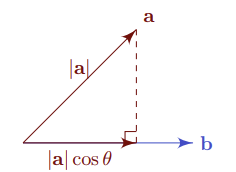
\includegraphics[width=5cm]{LA_ch1_dotproduct.png}
\end{figure}
However, this is only one of many possible scalar products, or \it inner products $\langle\mathbf{x|y}\rangle$, \normalfont that can be defined. Similar to a dot product, they are defined by the following properties:
\begin{enumerate}
    \item Commutativity: $\mathbf{\langle x|y\rangle=\langle y|x\rangle}$
    \item Distributive and associative properties: $\langle\mathbf{x}|(\lambda\mathbf{y}+\mu\mathbf{z})\rangle=\lambda\langle\mathbf{x|y}\rangle+ \mu\langle\mathbf{x|z}\rangle$
    \item Identity: if $\mathbf{\langle x|x\rangle=0}$, then $\mathbf{x}=0$; $\mathbf{\langle x|x\rangle}\geq 0$.
\end{enumerate}
Accordingly, we define the \it norm \normalfont of a vector $\mathbf{x}$ as follows:
\begin{definition}
    (Norm). The \it norm \normalfont of a vector $\mathbf{x}$ is defined as 
    \begin{equation}
        |\mathbf{x}|=\sqrt{\langle\mathbf{x}|\mathbf{x}\rangle}
    \end{equation}
\end{definition}
The above definitions encompasse far more than the dot product; for instance, if we define the vector space $V$ as the set of all real integrable functions $f(x)$, then we can verify that the operation 
\begin{equation}
    \langle f(x)|g(x) \rangle = \int_{0}^{1} f(x)g(x)\ dx
\end{equation}
is a valid inner product. This generality will be useful in establishing the power of the following result.
\subsection{Cauchy-Schwarz Inequality}
\begin{theorem}
    (Cauchy-Schwarz inequality). For all vectors $\mathbf{x,y}\in\mathbb{R^n}$, we have 
    \begin{equation}
        |\langle \mathbf{x | y}\rangle| \leq |\mathbf{x}||\mathbf{y}|.
    \end{equation}
    In other words, the norm of the inner product is greater than or equal to the product of the norms. This applies to any inner product on any real vector space, as the proof below will demonstrate.
\end{theorem}
\begin{proof}
    Consider the norm $|(\mathbf{x}-\lambda\mathbf{y})|$, which is non-negative by definition. Thus its square
    \begin{equation*}
        (\mathbf{x}-\lambda\mathbf{y})\cdot (\mathbf{x}-\lambda\mathbf{y})
    \end{equation*}
    is also non-negative, leading to 
    \begin{equation*}
        |\mathbf{x}| - 2\lambda \mathbf{x\cdot y} +\lambda^2 |\mathbf{y}| \geq 0
    \end{equation*}
    where $\cdot$ denotes any inner product. Reorganizing this as a quadratic equation in $\lambda$ and recognizing that it has at least one real solution, we have its discriminant
    \begin{equation*}
        \Delta = b^2-4ac=(4\mathbf{(x\cdot y)}^2) - 4|\mathbf{x||y|}\geq 0
    \end{equation*}
    leading to the desired result.
\end{proof}
We derived this proof entirely based on the axiomatic properties of inner products instead of a specific inner product (e.g. the dot product), so this inequality is applicable across any inner product in any real vector space - like the integral-based one defined above.
\subsection{Vector product}
Similar to the scalar product, we can also define a binary operation known as the \it vector product \normalfont over a vector space that takes two vectors and outputs another vector, 

\end{document}